\documentclass[10pt]{article}

\usepackage{amsmath}
\usepackage{amsthm}
\usepackage{amssymb}
\usepackage{graphicx}
\usepackage{tikz}
\usetikzlibrary{positioning,arrows.meta}
\usepackage[margin=1in]{geometry}
\usepackage{enumitem}
\usepackage{hyperref}
\usepackage{xcolor}

\hypersetup{
  colorlinks=true,
  linkcolor=blue,
  urlcolor=blue,
}

% ==========================================================
% Paper-code and person-code system
% ----------------------------------------------------------
% \papercode{KEY}      green [KEY] tag (non-clickable)
% \papercoderef{KEY}   green [KEY] that hyperlinks to \label{paper:KEY}
% \papercodehead{KEY}  bold green [KEY] for use as a list-item heading
%
% \personcode{KEY}     purple [KEY] tag (non-clickable)
% \personcoderef{KEY}  purple [KEY] that hyperlinks to \label{person:KEY}
%
% \pmrl{Label.}        italic underlined run-in label
%                      (e.g. \pmrl{Problem.}, \pmrl{Result.})
%
% To create a navigation anchor for a paper entry, start that entry with:
%   \phantomsection\label{paper:KEY}
% For a person entry:
%   \phantomsection\label{person:KEY}
% ==========================================================

\definecolor{papergreen}{RGB}{0,120,60}
\newcommand{\papercode}[1]{\textcolor{papergreen}{\texttt{[#1]}}}
\newcommand{\papercodehead}[1]{\textbf{\papercode{#1}}}
\definecolor{personpurple}{RGB}{100,40,140}
\newcommand{\personcode}[1]{\textcolor{personpurple}{\texttt{[#1]}}}
\newcommand{\pmrl}[1]{\underline{\textit{#1}}}

\newtheorem{thm}{Theorem}[section]
\newtheorem{lem}[thm]{Lemma}

\newcommand{\papercoderef}[1]{\hyperref[paper:#1]{\papercode{#1}}}
\newcommand{\personcoderef}[1]{\hyperref[person:#1]{\personcode{#1}}}

\title{[Research Group / Topic] Survey}
\author{[Author Name]}
\date{[Month Year]}

\begin{document}

\maketitle
\tableofcontents
\newpage

% ==========================================================
\section{Scope}
% ==========================================================

[One paragraph describing the purpose of this survey/report: whose work
is being surveyed, what the goal is, and what research direction it
supports. Mention which open problems you are trying to identify.]

% ==========================================================
\section{People}
% ==========================================================

This section introduces the researchers in the [Research Line].

% ----------------------------------------------------------
\subsection{Principal Investigators}
% ----------------------------------------------------------

\begin{itemize}[leftmargin=*]

\item \phantomsection\label{person:PI1}\personcode{PI1}
\textbf{[PI Full Name]}
(\href{https://example.com}{website},
\href{https://scholar.google.com}{Google Scholar})

[Brief description of research focus and why this person is relevant.]

\end{itemize}

% ----------------------------------------------------------
\subsection{Students and Trainees}
% ----------------------------------------------------------

\begin{itemize}[leftmargin=*]

\item \phantomsection\label{person:S1}\personcode{S1}
\textbf{[Student Full Name]}
(\href{https://example.com}{website};
[Year]--now PhD, [Institution])

Focus: [describe research focus].

\pmrl{Note.} [Why this person and their work are directly relevant to
your research direction. Be specific.]

\item \phantomsection\label{person:S2}\personcode{S2}
\textbf{[Student Full Name]}
(\href{https://scholar.google.com}{Google Scholar};
[Year]--now PhD, [Institution])

Focus: [describe research focus].

\pmrl{Note.} [Relevance note.]

\end{itemize}

% ----------------------------------------------------------
\subsection{Collaborators}
% ----------------------------------------------------------

\begin{itemize}[leftmargin=*]

\item \phantomsection\label{person:C1}\personcode{C1}
\textbf{[Collaborator Full Name]}
(\href{https://scholar.google.com}{Google Scholar}; [Institution])

Focus: [describe research focus].

\pmrl{Note.} [Relevance note.]

\end{itemize}

% ==========================================================
\section{Literature Map}
% ==========================================================

[Narrative paragraph: how the papers in this line relate to each other
and how they evolved. Use \papercoderef{...} to reference papers inline.
For example: ``The framework originated with \papercoderef{P1}, which
introduced X. Building on it, \papercoderef{P2} extended Y, and
\papercoderef{P3} applied it to Z.'']

The citation graph below maps the dependency structure of this literature.

\begin{center}
\resizebox{0.8\textwidth}{!}{%
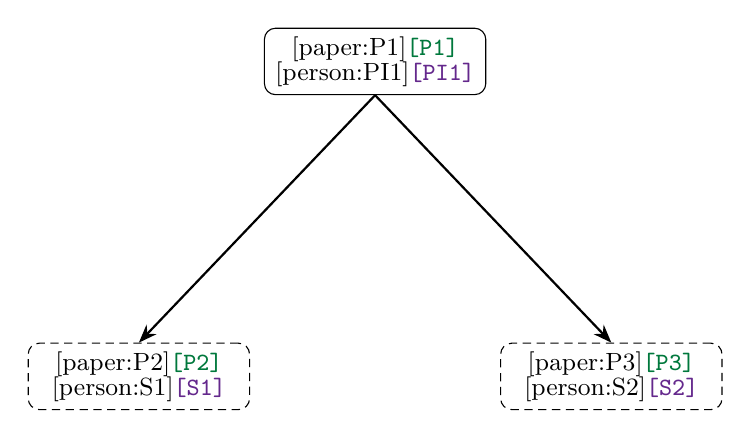
\begin{tikzpicture}[
  box/.style={draw, rounded corners, text width=2.6cm, align=center,
              font=\small, inner sep=3pt},
  ext/.style={draw, rounded corners, text width=2.6cm, align=center,
              font=\small, inner sep=3pt, densely dashed},
  arr/.style={-{Stealth}, thick}
]
  % Replace these nodes with your actual papers.
  % Solid box = core paper. Densely dashed = extension. Dashed = application.
  \node[box] (p1) at ( 0,  0) {\papercoderef{P1}\\[-2pt]
    {\small\personcoderef{PI1}}};
  \node[ext]  (p2) at (-3, -4) {\papercoderef{P2}\\[-2pt]
    {\small\personcoderef{S1}}};
  \node[ext]  (p3) at ( 3, -4) {\papercoderef{P3}\\[-2pt]
    {\small\personcoderef{S2}}};
  \draw[arr] (p1.south) -- (p2.north);
  \draw[arr] (p1.south) -- (p3.north);
\end{tikzpicture}%
}
\end{center}
\noindent\small Arrow $A\to B$: $B$ builds directly on $A$.
Solid: core paper. Densely dashed: extension.\normalsize

% ----------------------------------------------------------
\subsection{Core Papers}
% ----------------------------------------------------------

\begin{itemize}[leftmargin=*]

\item \phantomsection\label{paper:P1}\papercodehead{P1}
[Author(s)].
\emph{[Title]}.
\emph{[Journal or Conference]}, [Year].
\href{https://doi.org/...}{Publisher link}
(\href{https://arxiv.org/abs/...}{arXiv:XXXX.XXXXX}).

\pmrl{Problem.} [What problem does this paper address?]

\pmrl{Method.} [What is the main technical approach? Include key
equations if they are central to understanding the result.]

\pmrl{Result.} [What is the main result? Be precise about
what is proved and in which norm or setting.]

\pmrl{Limitation.} [What assumptions or open questions remain?]

\end{itemize}

% ----------------------------------------------------------
\subsection{Extensions}
% ----------------------------------------------------------

\begin{itemize}[leftmargin=*]

\item \phantomsection\label{paper:P2}\papercodehead{P2}
[Author(s)].
\emph{[Title]}.
\emph{[Journal or Conference]}, [Year].
\href{https://doi.org/...}{Publisher link}
(\href{https://arxiv.org/abs/...}{arXiv:XXXX.XXXXX}).

\pmrl{Problem.} [...]

\pmrl{Method.} [...]

\pmrl{Result.} [...]

\pmrl{Limitation.} [...]

\item \phantomsection\label{paper:P3}\papercodehead{P3}
[Author(s)].
\emph{[Title]}.
\emph{[Journal or Conference]}, [Year].
\href{https://doi.org/...}{Publisher link}.

\pmrl{Problem.} [...]

\pmrl{Method.} [...]

\pmrl{Result.} [...]

\end{itemize}

% ==========================================================
\section{Research Directions}\label{sec:directions}
% ==========================================================

% ----------------------------------------------------------
\subsection{[Direction 1 Title]}
% ----------------------------------------------------------

[Describe the open problem. State clearly what the existing literature
does not address. Explain how your tools, background, or perspective
could contribute. Be concrete: name the specific model, equation, or
mechanism you would study.]

% ----------------------------------------------------------
\subsection{[Direction 2 Title]}
% ----------------------------------------------------------

[...]

% ==========================================================
\section*{References}
% ==========================================================

\begin{itemize}[leftmargin=*]

\item \phantomsection\label{paper:P1_ref}\papercodehead{P1}
[Author(s)].
\emph{[Title]}.
\emph{[Journal or Conference]}, [Year].
\href{https://doi.org/...}{https://doi.org/...}.

\item \phantomsection\label{paper:P2_ref}\papercodehead{P2}
[Author(s)].
\emph{[Title]}.
\emph{[Journal or Conference]}, [Year].
\href{https://arxiv.org/abs/...}{arXiv:XXXX.XXXXX}.

\item \phantomsection\label{paper:P3_ref}\papercodehead{P3}
[Author(s)].
\emph{[Title]}.
\emph{[Journal or Conference]}, [Year].
\href{https://doi.org/...}{https://doi.org/...}.

\end{itemize}

\end{document}
